\documentclass[aspectratio=169,11pt]{beamer}

\usetheme{Boadilla}
\usecolortheme{default}
\usefonttheme{professionalfonts}
\setbeamertemplate{navigation symbols}{}
\setbeamertemplate{itemize items}[circle]
\setbeamertemplate{enumerate items}[default]
\definecolor{stanfordred}{RGB}{140,21,21}
\definecolor{darkgray}{RGB}{45,45,45}
\definecolor{softgray}{RGB}{245,245,245}
\setbeamercolor{structure}{fg=stanfordred}
\setbeamercolor{title}{fg=stanfordred}
\setbeamercolor{frametitle}{fg=stanfordred}
\setbeamercolor{block title}{bg=stanfordred!10,fg=stanfordred}
\setbeamercolor{block body}{bg=softgray,fg=black}
\setbeamercolor{footline}{fg=darkgray,bg=white}

\usepackage[T1]{fontenc}
\usepackage[utf8]{inputenc}
\usepackage{lmodern}
\usepackage{amsmath,amssymb,mathtools}
\usepackage{booktabs}
\usepackage{tikz}
\usetikzlibrary{positioning}
\usepackage{array}
\usepackage{pifont}
\usepackage{hyperref}
\hypersetup{colorlinks=true,urlcolor=stanfordred,linkcolor=stanfordred}

\newcommand{\R}{\mathcal{R}}
\newcommand{\J}{\mathcal{J}}
\newcommand{\A}{\mathsf{A}}
\newcommand{\Q}{\mathsf{Q}}
\newcommand{\Lrank}{\mathsf{L}}
\newcommand{\alphQ}{\alpha_{\Q}}
\newcommand{\source}[1]{{\scriptsize\color{darkgray}#1}}
\newcommand{\yes}{\textcolor{stanfordred}{\ding{72}}}

\title[Inverting Path Compression]{Inverting Path Compression}
\subtitle{A proof-digestion case study}
\author[Don Poindexter]{Don Poindexter}
\institute[Stanford AI for Lean4 Club]{Stanford AI for Lean4 Club}
\date{After Seidel--Sharir (2005) and Tarjan's Dagstuhl prompt (2025)}

\setbeamertemplate{footline}{%
  \leavevmode%
  \hbox{%
  \begin{beamercolorbox}[wd=.72\paperwidth,ht=2.4ex,dp=1ex,leftskip=1.5em]{footline}%
    \insertshorttitle
  \end{beamercolorbox}%
  \begin{beamercolorbox}[wd=.28\paperwidth,ht=2.4ex,dp=1ex,rightskip=1.5em plus1fil]{footline}%
    \hfill\insertframenumber/\inserttotalframenumber
  \end{beamercolorbox}}%
  \vskip0pt%
}


\begin{document}

\begin{frame}[plain]
  \centering
  \vspace{0.5cm}
  {\Large \textsc{Stanford AI for Lean4 Club}}\\[1.0cm]
  {\usebeamerfont{title}\usebeamercolor[fg]{title}\Huge Inverting Path Compression}\\[0.25cm]
  {\Large a proof-digestion case study}\\[0.8cm]
  \begin{block}{}
  \centering
  \Large Invert the Seidel--Sharir shrinkers; the recursion becomes Ackermann growth.
  \end{block}
  \vfill
  {\large Don Poindexter}\\[0.15cm]
  {\small After Seidel--Sharir (2005), Tarjan's Dagstuhl prompt (2025), and a targeted prior-art audit}
\end{frame}

\begin{frame}{TL;DR: the whole story}
\framesubtitle{A proof-digestion loop around a concrete mathematical prompt}
\begin{center}
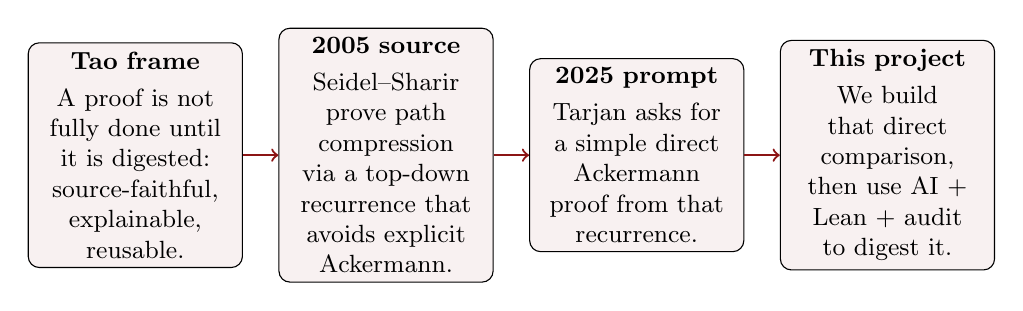
\begin{tikzpicture}[
  node distance=0.45cm,
  every node/.style={font=\small},
  box/.style={draw,rounded corners,fill=stanfordred!6,minimum width=0.22\textwidth,text width=0.205\textwidth,align=center,minimum height=2.05cm},
  arrow/.style={->,thick,stanfordred}
]
  \node[box] (tao) {\textbf{Tao frame}\\[0.08cm]
  A proof is not fully done until it is digested: source-faithful, explainable, reusable.};
  \node[box,right=of tao] (source) {\textbf{2005 source}\\[0.08cm]
  Seidel--Sharir prove path compression via a top-down recurrence that avoids explicit Ackermann.};
  \node[box,right=of source] (prompt) {\textbf{2025 prompt}\\[0.08cm]
  Tarjan asks for a simple direct Ackermann proof from that recurrence.};
  \node[box,right=of prompt] (ours) {\textbf{This project}\\[0.08cm]
  We build that direct comparison, then use AI + Lean + audit to digest it.};
  \draw[arrow] (tao) -- (source);
  \draw[arrow] (source) -- (prompt);
  \draw[arrow] (prompt) -- (ours);
\end{tikzpicture}
\end{center}
\vspace{0.25cm}
\begin{block}{High-level punchline}
\centering
\Large Invert the rank-shrinkers. In the inverted coordinates, Seidel--Sharir's recursive shrinker becomes Ackermann growth.
\end{block}
\end{frame}

\begin{frame}{Where the problem comes from}
\framesubtitle{Seidel--Sharir supplied the recurrence; Tarjan asked for the direct Ackermann bridge}
\begin{columns}[T,totalwidth=\textwidth]
\begin{column}{0.48\textwidth}
\begin{block}{2005: Seidel--Sharir}
\textit{Top-Down Analysis of Path Compression}, SIAM J. Comput. 34(3), 515--525.
\medskip

They give a top-down recurrence based on a hierarchy $J_k$; their abstract says the inverse-Ackermann bound follows \emph{without having to introduce the Ackermann function itself}.
\end{block}
\source{Source: Seidel--Sharir, DOI 10.1137/S0097539703439088.}
\end{column}
\begin{column}{0.48\textwidth}
\begin{block}{2025: Tarjan at Dagstuhl 25191}
The Dagstuhl summary records that Tarjan drew attention to different analyses of path compression and raised the question of an alternative proof.
\medskip

Section 5.3 points back to the Seidel--Sharir recurrence and asks for the direct classical-Ackermann connection.
\end{block}
\source{Source: Dagstuhl Seminar 25191 report page and Section 5.3.}
\end{column}
\end{columns}
\vspace{0.35cm}
\begin{center}
\Large The task is to \textbf{connect Seidel--Sharir's $J$ hierarchy directly to classical Ackermann growth.}
\end{center}
\end{frame}

\begin{frame}{Why believe this is a live prompt?}
\framesubtitle{The targeted novelty search found adjacent routes; this bridge was not located}
\small
\begin{center}
\begin{tabular}{>{\raggedright\arraybackslash}p{0.30\textwidth}>{\raggedright\arraybackslash}p{0.30\textwidth}>{\raggedright\arraybackslash}p{0.30\textwidth}}
\toprule
\textbf{Source family} & \textbf{What it gives} & \textbf{Gap relative to this route}\\
\midrule
Tarjan-style analyses & Classical Ackermann appears directly in a bottom-up analysis. & Uses classical $A$ directly, rather than passing through the Seidel--Sharir $J^\diamond$ recurrence.\\[0.10cm]
Seidel--Sharir / Seidel & A top-down $J$-hierarchy that makes the bound natural. & Keeps the story internal to the $J$-hierarchy, rather than proving a quantitative $J\to A$ bridge.\\[0.10cm]
Modern simplifications and formalizations & Cleaner union-find proofs and verified analyses. & Works in other frameworks rather than the route $J_k\mapsto R_k\mapsto A$.\\
\bottomrule
\end{tabular}
\end{center}
\vspace{0.25cm}
\begin{block}{Cautious conclusion}
The targeted audit found many adjacent analyses, but no public source with the specific threshold-inversion route used here.
\end{block}
\end{frame}

\begin{frame}{What specific bridge was missing?}
\framesubtitle{The object and inequality that make the direct comparison work}
\begin{block}{The new coordinate}
For the Seidel--Sharir hierarchy, define the max-inverse
\[
  R_k(t)=\max\{r\ge 0:J_k(r)\le t\}.
\]
This asks: at level $k$, how large a rank can be pushed below threshold $t$?
\end{block}
\vspace{0.15cm}
\begin{block}{The direct bridge to classical Ackermann}
The proof note shows
\[
  R_{z+1}(Q)\ge A(z,4Q)
  \qquad (z\ge 1,\; Q\ge 1).
\]
So the Seidel--Sharir shrinkers dominate classical Ackermann growth after inversion.
\end{block}
\vspace{0.1cm}
\begin{center}
\small Evidence-based claim: public prior-art search found no source proving this bridge for $J^\diamond$.
\end{center}
\end{frame}

\begin{frame}{Why this belongs in a Lean/AI club}
\framesubtitle{Tao's proof-digestion frame: three jobs; the third is the least automatic}
\begin{center}
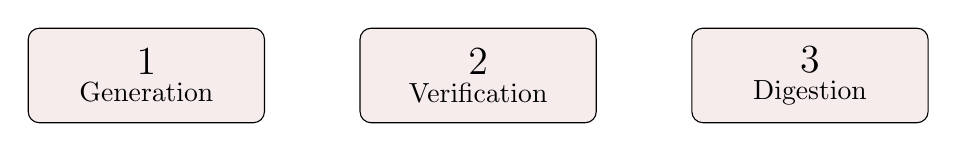
\begin{tikzpicture}[node distance=1.2cm]
  \node[draw,rounded corners,fill=stanfordred!8,minimum width=3.0cm,minimum height=1.2cm] (gen) {\shortstack{\Large 1\\Generation}};
  \node[draw,rounded corners,fill=stanfordred!8,minimum width=3.0cm,minimum height=1.2cm,right=1.2cm of gen] (ver) {\shortstack{\Large 2\\Verification}};
  \node[draw,rounded corners,fill=stanfordred!8,minimum width=3.0cm,minimum height=1.2cm,right=1.2cm of ver] (dig) {\shortstack{\Large 3\\Digestion}};
\end{tikzpicture}
\end{center}
\vspace{0.3cm}
\begin{block}{Talk thesis}
This talk is about using AI, Lean, and red-team audit to support digestion without outsourcing judgment. The math is the example; the meta-claim is the workflow.
\end{block}
\vspace{0.2cm}
\begin{center}
\Large ``A theorem is not done until it is source-faithful, narratable, and reusable.''
\end{center}
\end{frame}

\begin{frame}{Minimal background}
\framesubtitle{Enough vocabulary to read the recurrence}
\begin{columns}[T,totalwidth=\textwidth]
\begin{column}{0.48\textwidth}
\begin{block}{Path compression}
Union--find stores each set as a rooted tree. A find operation walks from a node to the root, then rewires the visited nodes closer to the root.
\medskip

The analysis counts the total cost of many such compressions.
\end{block}
\end{column}
\begin{column}{0.48\textwidth}
\begin{block}{Ranks and the cost function}
Ranks measure how high a node can sit in the forest. Let
\[
  f(m,n,r)
\]
be the worst-case cost of $m$ compressions on $n$ nodes when the maximum rank is at most $r$.
\end{block}
\end{column}
\end{columns}
\vspace{0.25cm}
\begin{block}{What Seidel--Sharir add}
They build a hierarchy $J_0,J_1,J_2,\ldots$ of rank-shrinking functions. If $J_k(r)$ is small, the recurrence gives a good cost bound.
\end{block}
\end{frame}

\begin{frame}{The setup}
\framesubtitle{The Seidel--Sharir hierarchy, written explicitly}
\begin{block}{Start with a simple rank shrinker}
\[
  J_0(r)=\left\lceil\frac{r-1}{2}\right\rceil.
\]
\end{block}

\begin{block}{The diamond operation}
For any shrinker $g$, define a new shrinker $g^\diamond$ by
\[
  g^\diamond(r)=
  \begin{cases}
    g(r), & g(r)\le 1,\\[0.15cm]
    1+g^\diamond\!\left(\left\lceil\log_2 g(r)\right\rceil\right), & g(r)>1.
  \end{cases}
\]
Then Seidel--Sharir set $J_{k+1}=J_k^\diamond$.
\end{block}
\end{frame}

\begin{frame}{What the recurrence asks us to prove}
\framesubtitle{The path-compression bound is reduced to understanding how fast $J_k$ shrinks}
\begin{center}
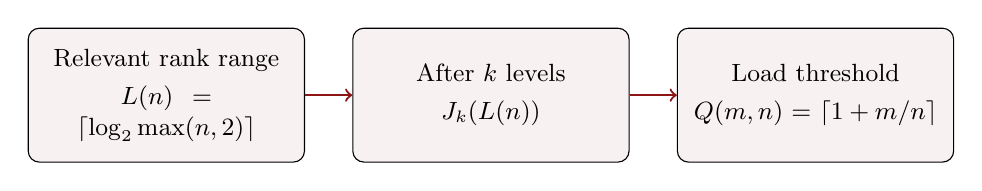
\begin{tikzpicture}[
  every node/.style={font=\small},
  box/.style={draw,rounded corners,fill=stanfordred!6,text width=0.27\textwidth,align=center,minimum height=1.7cm},
  arrow/.style={->,thick,stanfordred}
]
  \node[box] (rank) {Relevant rank range\\[0.1cm] $L(n)=\lceil\log_2\max(n,2)\rceil$};
  \node[box,right=0.6cm of rank] (shrink) {After $k$ levels\\[0.1cm] $J_k(L(n))$};
  \node[box,right=0.6cm of shrink] (threshold) {Load threshold\\[0.1cm] $Q(m,n)=\left\lceil 1+m/n\right\rceil$};
  \draw[arrow] (rank) -- (shrink);
  \draw[arrow] (shrink) -- (threshold);
\end{tikzpicture}
\end{center}
\vspace{0.25cm}
\begin{block}{Cost recurrence}
\[
  f(m,n,r) \le k\,m + 2n\,J_k(r).
\]
So once $J_k(r)$ is small, the cost bound follows.
\end{block}
\vspace{0.15cm}
\begin{block}{Core question}
\centering
How small does $k$ need to be before
\[
  J_k(L(n))\le Q(m,n)?
\]
\end{block}
\end{frame}

\begin{frame}{The trick: invert shrinking into reach}
\framesubtitle{Comparing a shrinker to a grower directly fights the objects}
\begin{columns}[T,totalwidth=\textwidth]
\begin{column}{0.48\textwidth}
\begin{block}{Shrink view}
Given rank $r$, how small does level $k$ make it?
\[
  r \longmapsto J_k(r).
\]
\end{block}
\end{column}
\begin{column}{0.48\textwidth}
\begin{block}{Reach view: the digestion move}
Given threshold $t$, how far up does level $k$ reach?
\[
  R_k(t)=\max\{r\ge 0: J_k(r)\le t\}.
\]
\end{block}
\end{column}
\end{columns}
\vspace{0.45cm}
\begin{center}
\Large Base row is exact:
\[
  R_0(t)=2t+1,
  \qquad
  J_0(r)\le t \iff r\le 2t+1.
\]
\end{center}
\end{frame}

\begin{frame}{The engine}
\framesubtitle{The diamond recursion becomes row-by-row exponential amplification}
On the recursive branch $J_k(r)>1$:
\[
  J_{k+1}(r)=1+J_{k+1}\!\left(\left\lceil\log_2 J_k(r)\right\rceil\right).
\]

To prove $J_{k+1}(r)\le t+1$, it suffices that
\[
  \left\lceil\log_2 J_k(r)\right\rceil \le R_{k+1}(t),
\]
which is forced by
\[
  J_k(r)\le 2^{R_{k+1}(t)}.
\]

\begin{block}{Threshold step}
\[
  R_{k+1}(t+1) \ge R_k\!\left(2^{R_{k+1}(t)}\right).
\]
\end{block}
\begin{center}
One extra threshold unit at level $k+1$ buys an exponentially larger input threshold at level $k$.
\end{center}
\end{frame}

\begin{frame}{Why Ackermann appears}
\framesubtitle{Row-feeding recurrence + Ackermann recursion: same structural shape}
\begin{block}{Row domination}
\[
  R_j(x) \ge A(j+1,x)
  \qquad (j\ge 1,\; x\ge 1).
\]
\end{block}

\begin{block}{Main comparison: the answer to Tarjan's prompt}
\[
  R_{z+1}(Q) \ge A(z,4Q)
  \qquad (z\ge 1,\; Q\ge 1).
\]
\end{block}

\begin{block}{Where the $4Q$ comes from}
For $Q\ge 2$:
\[
\begin{aligned}
R_{k+1}(Q) &\ge R_k\!\left(2^{R_{k+1}(Q-1)}\right),\\
R_{k+1}(Q-1) &\ge R_0(Q-1)=2Q-1,\\
2^{2Q-1} &\ge 4Q.
\end{aligned}
\]
\end{block}
\source{The $Q=1$ endpoint is handled separately in the proof note.}
\end{frame}

\begin{frame}{Closing the cost bound}
\framesubtitle{Choose the Ackermann row that clears the rank range; plug into the source recurrence}
\[
  L(n)=\left\lceil\log_2\max(n,2)\right\rceil,
  \qquad
  Q(m,n)=\left\lceil 1+\frac{m}{n}\right\rceil.
\]
\[
  \alpha_Q(m,n)=\min\{z\ge 1: A(z,4Q(m,n))>L(n)\}.
\]

\begin{block}{Main comparison gives}
\[
  J_{z+1}(L(n))\le Q(m,n)
  \qquad\text{for }z=\alpha_Q(m,n).
\]
\end{block}

\begin{block}{Therefore}
\[
  f(m,n,L(n))\le (\alpha_Q(m,n)+3)m+4n
  =O\!\left(m\,\alpha_Q(m,n)+n\right).
\]
\end{block}
\source{For the real source threshold $1+m/n$, the nonintegral case costs at most one extra level.}
\end{frame}

\begin{frame}{The proof spine}
\framesubtitle{Everything exists to support the threshold step and the main comparison}
\small
\begin{center}
\begin{tabular}{>{\raggedright\arraybackslash}p{0.82\textwidth}c}
\toprule
Source recurrence $f\le k m+2nJ_k(r)$ & \\
Source hierarchy $J_0=\lceil(r-1)/2\rceil$, $J_{k+1}=J_k^\diamond$ & \\
Basic $J$ package: monotone, unbounded, $J_{k+1}\le J_k$, $R_k$ finite & \\
\textbf{Threshold step} $R_{k+1}(t+1)\ge R_k(2^{R_{k+1}(t)})$ & \yes \\
Threshold jump $R_{k+1}(Q)\ge R_k(4Q)$ for $Q\ge 2$ & \\
Row domination $R_j(x)\ge A(j+1,x)$ for $j,x\ge 1$ & \\
\textbf{Main comparison} $R_{z+1}(Q)\ge A(z,4Q)$ for $z,Q\ge 1$ & \yes \\
Alpha/cost consequence $f(m,n,L(n))\le (\alpha_Q+3)m+4n$ & \\
\bottomrule
\end{tabular}
\end{center}
\vspace{0.15cm}
\begin{center}
\yes\; = the two slides everything else exists to support.
\end{center}
\end{frame}

\begin{frame}{Lesson 1. Digestion is the bottleneck}
\framesubtitle{AI generates artifacts cheaply. The bottleneck is the story that survives audit.}
\begin{columns}[T,totalwidth=\textwidth]
\begin{column}{0.48\textwidth}
\begin{block}{Raw workflow produced}
\begin{itemize}
  \item prompts
  \item proof notes $(v0.1.0\to v0.1.4)$
  \item adversarial audits
  \item source-anchor packet
  \item finite sanity-check script
  \item Lean formalization branches
  \item Codex worker traces
\end{itemize}
\end{block}
\end{column}
\begin{column}{0.48\textwidth}
\begin{block}{What survives}
\centering
\Large
Invert the Seidel--Sharir shrinkers; diamond becomes Ackermann growth.
\end{block}
\vspace{0.3cm}
The compression ratio matters: every hour of generation is wasted if no human can carry the result.
\end{column}
\end{columns}
\end{frame}

\begin{frame}[fragile]{Lesson 2. Formalization exposes architecture}
\framesubtitle{A ``primitive'' lemma turned out to be derived}
\begin{columns}[T,totalwidth=\textwidth]
\begin{column}{0.48\textwidth}
\begin{block}{Schematic before}
{\scriptsize
\begin{verbatim}
structure ThresholdAssumptions where
  baseExact
  monotoneThreshold
  monotoneLevel
  thresholdStep
  thresholdJump  -- primitive
\end{verbatim}
}
\end{block}
\end{column}
\begin{column}{0.48\textwidth}
\begin{block}{Schematic after}
{\scriptsize
\begin{verbatim}
structure ThresholdCoreAssumptions where
  baseExact
  monotoneThreshold
  monotoneLevel
  thresholdStep

theorem threshold_jump_from_step :
  -- derived from core assumptions
\end{verbatim}
}
\end{block}
\end{column}
\end{columns}
\vspace{0.2cm}
\begin{center}
\Large A ``magic move'' became a structural consequence. That is proof digestion in its strongest form.
\end{center}
\source{Commit milestone: b29a6a9.}
\end{frame}

\begin{frame}{Lesson 3. Honest boundaries}
\framesubtitle{What is machine-checked, and what is still a paper bridge?}
\begin{columns}[T,totalwidth=\textwidth]
\begin{column}{0.48\textwidth}
\begin{block}{Lean-checked: abstract engine}
\small
\begin{itemize}
  \item packet Ackermann lemmas
  \item row-domination invariant under \texttt{ThresholdCoreAssumptions}
  \item threshold jump derived from threshold step + monotonicity + base exactness
  \item main comparison $A(z,4Q)\le R(z+1,Q)$ for $z,Q\ge 1$
\end{itemize}
\end{block}
\end{column}
\begin{column}{0.48\textwidth}
\begin{block}{Paper-only: concrete bridge}
\small
\begin{itemize}
  \item concrete $J_0$ and $J_{k+1}=J_k^\diamond$
  \item concrete inverse $R_k(t)=\max\{r:J_k(r)\le t\}$
  \item proof that concrete $R$ satisfies \texttt{ThresholdCoreAssumptions}
  \item $\alpha_Q$, $\alpha_J^Q$, $\alpha_J^S$, and cost consequence
\end{itemize}
\end{block}
\end{column}
\end{columns}
\vspace{0.2cm}
\begin{center}
\Large Strategic target: concrete $R\Rightarrow$ \texttt{ThresholdCoreAssumptions}.\\
\normalsize First steps: define concrete $J_0$, \texttt{diamond}, and concrete $R_k$.
\end{center}
\end{frame}

\begin{frame}{Two things to remember}
\begin{block}{Mathematical TL;DR}
\centering
\Large Invert the Seidel--Sharir shrinkers; diamond becomes Ackermann growth.
\end{block}
\vspace{0.35cm}
\begin{block}{Proof-digestion TL;DR}
\centering
\Large Lean and adversarial audit helped separate the proof into a checked abstract engine and an explicit concrete bridge target.
\end{block}
\vfill
\begin{center}
\href{https://github.com/patternscientist/path-compression-digestion}{github.com/patternscientist/path-compression-digestion}\\[0.25cm]
Questions?
\end{center}
\end{frame}

\begin{frame}{Sources and reproducibility}
\small
\begin{itemize}
  \item Raimund Seidel and Micha Sharir, \textit{Top-Down Analysis of Path Compression}, SIAM J. Comput. 34(3):515--525, 2005. DOI: \href{https://doi.org/10.1137/S0097539703439088}{10.1137/S0097539703439088}.
  \item Robert E. Tarjan, ``Top-down analysis of path compression,'' in Dagstuhl Seminar 25191, \textit{Adaptive and Scalable Data Structures}, Dagstuhl Reports 15(5), 2025.
  \item Targeted novelty memo: prior-art search over Seidel--Sharir, Seidel slides/lectures, Tarjan-style analyses, modern simplifications, verified union-find work, and Dagstuhl follow-up traces.
  \item Project repository: \href{https://github.com/patternscientist/path-compression-digestion}{github.com/patternscientist/path-compression-digestion}. Start with the proof note, audit, sanity script, and source-anchor packet.
\end{itemize}
\vfill
\begin{block}{Novelty hygiene}
The deck states an evidence-based claim: a targeted public prior-art search found no source with this specific threshold-inversion bridge. It does not claim to rule out every private note, lecture, or unindexed thesis.
\end{block}
\end{frame}

\end{document}
